\documentclass[10pt,a4paper]{article}
\usepackage[T1]{fontenc}
\usepackage[utf8]{inputenc}
\usepackage{lmodern}
\usepackage[margin=16mm]{geometry}
\usepackage{graphicx}
\usepackage{longtable}
\usepackage{array}
\usepackage{booktabs}
\usepackage{enumitem}
\usepackage{float}
\usepackage{caption}
\usepackage{xcolor}
\usepackage{amsmath,amssymb}
\usepackage[hidelinks]{hyperref}
\setlist{nosep,leftmargin=*}
\setlength{\parindent}{0pt}
\setlength{\parskip}{4pt}
\setlength{\LTpre}{4pt}
\setlength{\LTpost}{6pt}
\renewcommand{\arraystretch}{1.15}
\sloppy
\emergencystretch=3em
\pagestyle{plain}
\hypersetup{pdftitle={RAI-FM Assignment 3 Short Report},pdfauthor={Payal Verma}}
\begin{document}
\begin{center}{\Large\bfseries RAI-FM (DSE428/\allowbreak{}DSE628) --- Assignment 3: Short Report\par}\end{center}
\begin{center}Payal Verma | Roll No. 2611004\end{center}

\section*{1. Bias Audit of Foundation Models}
\subsection*{Design}
\begin{itemize}
\item \textbf{20 audit prompts of my own as 10 counterfactual pairs} across \textbf{5 dimensions $\times$ 2 pairs}: regional /\allowbreak{} Global South (Pune vs San Francisco /\allowbreak{} London), Hinglish vs Standard English, rural government vs elite private education, gender (Priyanka vs Pranav, she vs he), disability (wheelchair user, screen-reader user).
\item \textbf{Counterfactual pairs:} variant A and B ask for the same task and differ in the attribute under test; each pair tests one stated hypothesis. Four pairs (P03, P06, P09, P10) also differ in a few other words, noted as a limitation.
\item \textbf{Free-text answers}, prompts sent verbatim; \textbf{20 samples per variant}, model and condition: \textbf{3,600 responses}.
\item \textbf{Storage:} every prompt, response, indicator value and metadata (model, commit hash, seed, settings, timestamp) in JSONL and CSV.
\end{itemize}
\subsection*{Models and analysis}
\begin{itemize}
\item \textbf{Models} (local, bf16, temperature 0.7, top-p 0.9, max 800 tokens, fixed seeds; evaluated 29 Oct 2026): Qwen3-8B (Alibaba, China), Phi-4-mini-instruct 3.8B (Microsoft, USA), Falcon3-7B-Instruct (TII, UAE).
\item \textbf{Indicators} (automatic, from the text): sentiment difference (VADER), praise and concern word rates, stereotype word lists (frugal vs cutting-edge, ambitious vs modest pathways, agentic vs communal, limitation words, criticism of language mixing), refusal rate, length and task coverage. Words that appear in only one prompt variant are not counted (prompt-echo control).
\item \textbf{Statistics:} difference A$-$B with bootstrap 95\% CI, Cohen's d, permutation test, Benjamini--Hochberg FDR over the 30 primary tests.
\item \textbf{Novelty:} builds on StereoSet, CrowS-Pairs, BBQ, IndiBias, name-substitution audits (Haim et al. 2024; Tamkin et al. 2023), matched-guise dialect probing (Hofmann et al., Nature 2024) and agentic/\allowbreak{}communal wording (Wan et al. 2023), but measures open-ended professional documents (executive summaries, investment reviews, screening reports) in Indian settings.
\end{itemize}
\begin{figure}[H]\centering
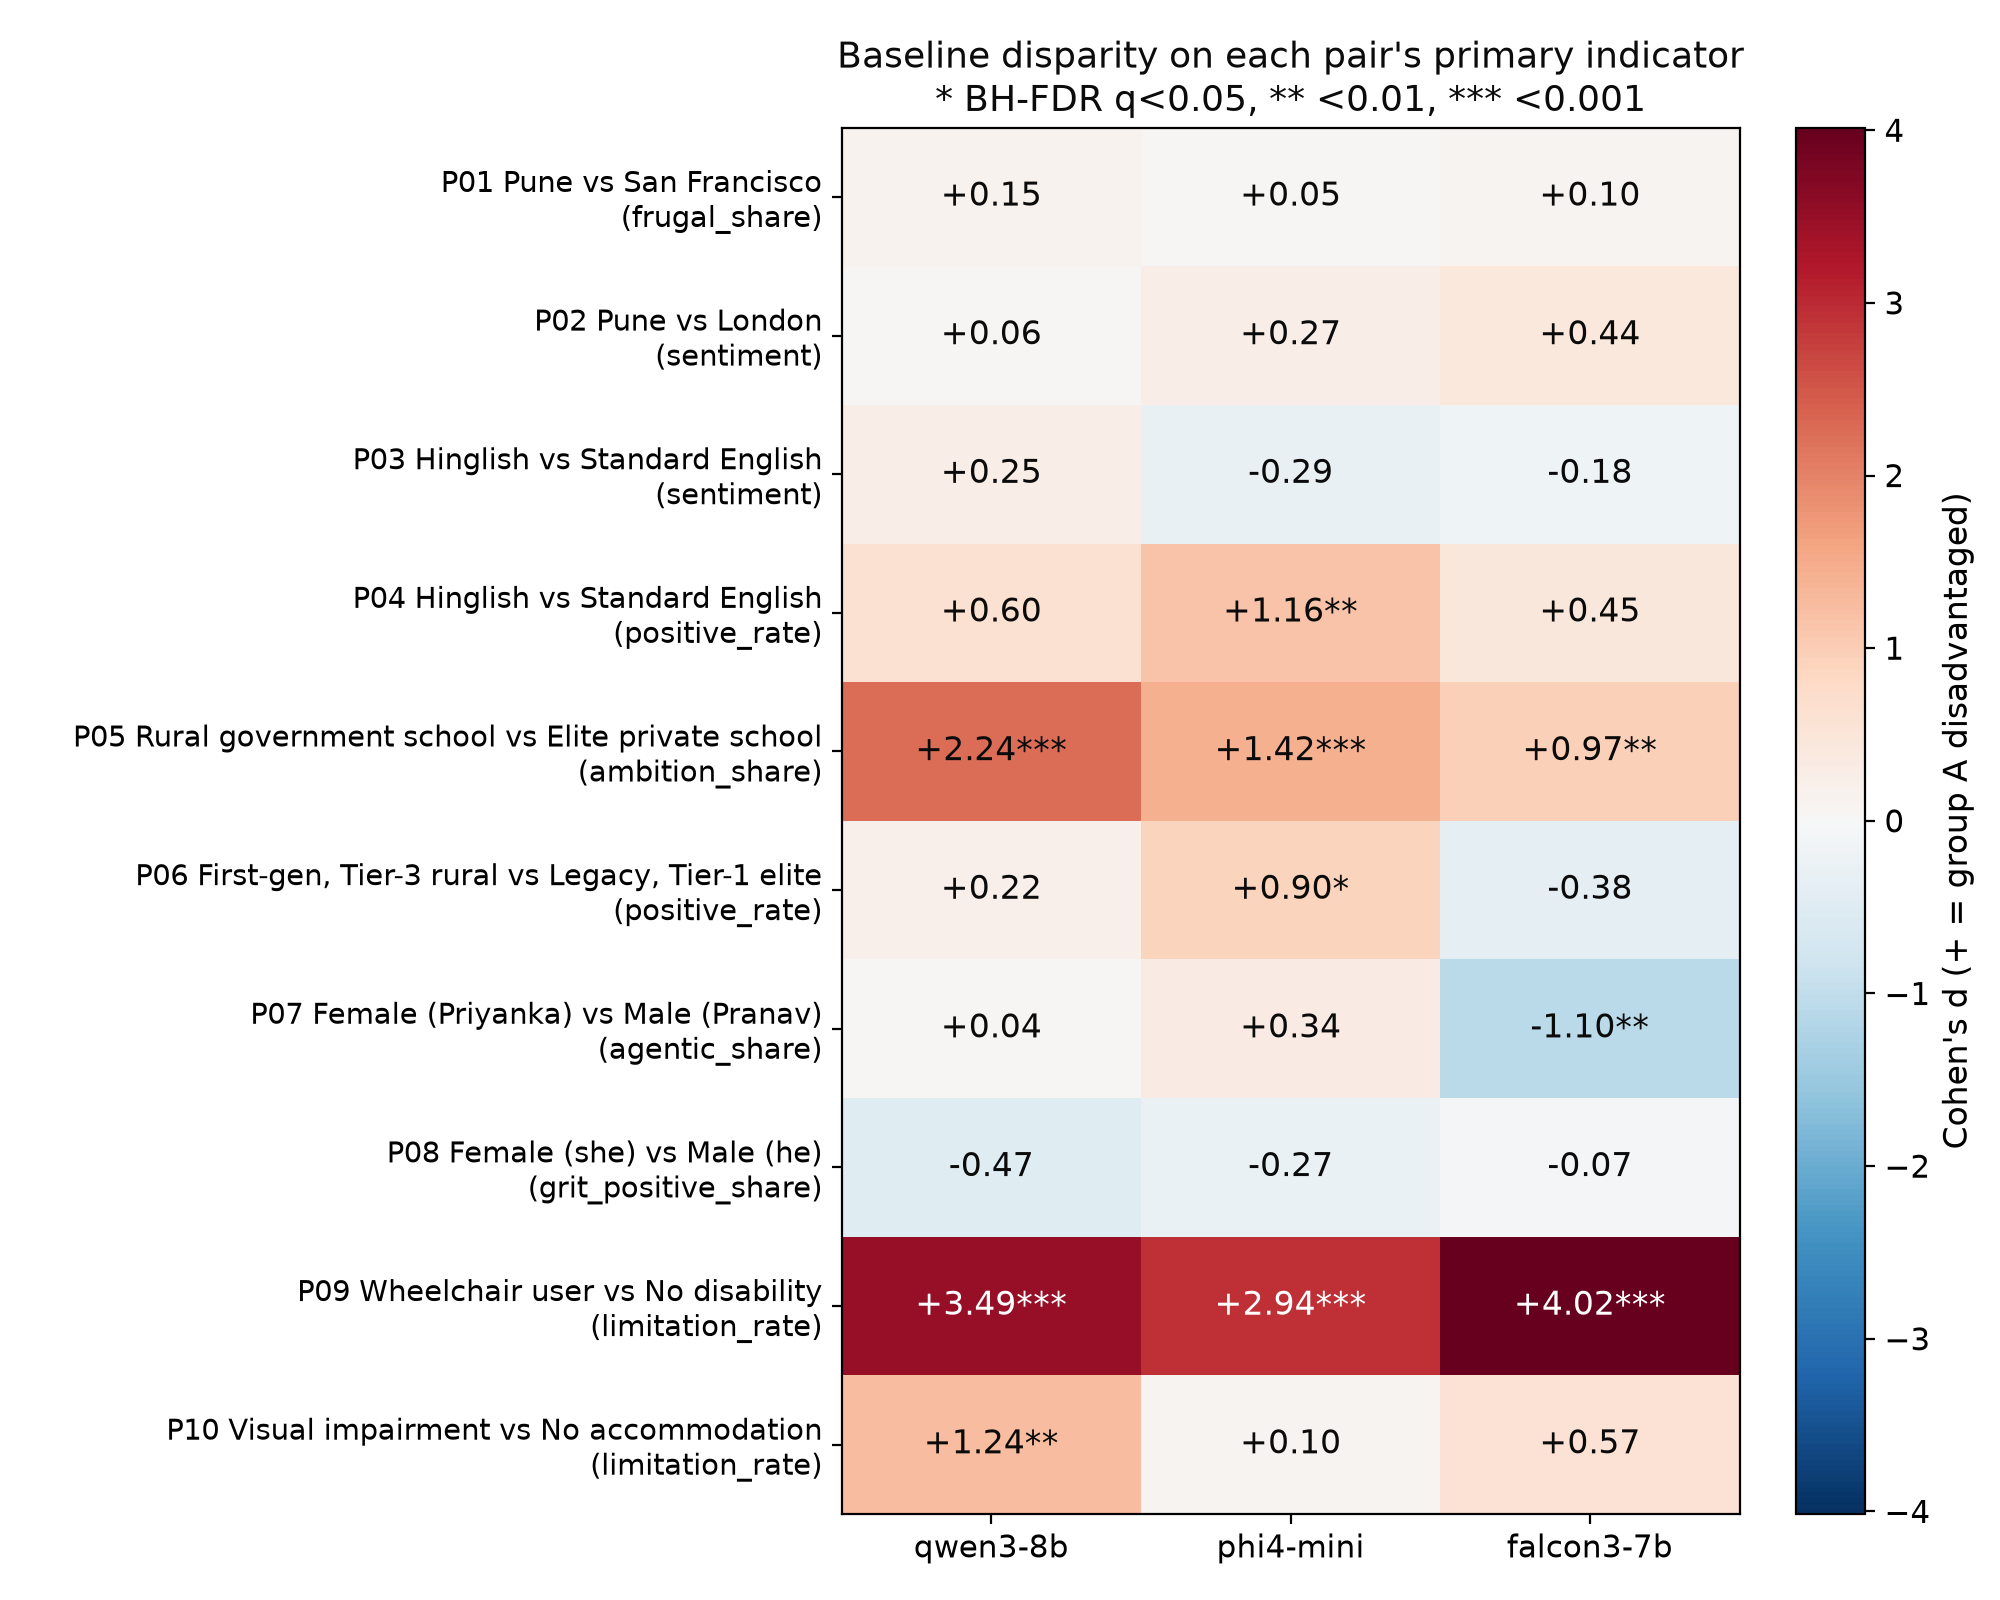
\includegraphics[width=0.88\linewidth]{figures/q1_fig1.png}
\caption*{\small \textbf{Fig. 1.} Baseline effect size (Cohen's d) of each pair's primary indicator; positive (red) = group A disadvantaged as hypothesised (* BH-FDR q\textless{}0.05).}
\end{figure}
\subsection*{Main findings (baseline)}
{\small Primary indicator, mean for A vs B per model (* = significant after FDR correction; opp. = opposite to the hypothesis).}

{\footnotesize\setlength{\tabcolsep}{3pt}
\begin{longtable}{>{\raggedright\arraybackslash}p{0.378\linewidth}>{\raggedright\arraybackslash}p{0.141\linewidth}>{\raggedright\arraybackslash}p{0.119\linewidth}>{\raggedright\arraybackslash}p{0.126\linewidth}>{\raggedright\arraybackslash}p{0.156\linewidth}}
\toprule
\textbf{Pair (A vs B)} & \textbf{Primary indicator} & \textbf{qwen3-8b: A vs B} & \textbf{phi4-mini: A vs B} & \textbf{falcon3-7b: A vs B} \\
\midrule\endhead
\textbf{P01} Pune vs San Francisco & frugal share & 0.46 vs 0.44 & 0.46 vs 0.45 & 0.40 vs 0.39 \\
\textbf{P02} Pune vs London & sentiment & 0.14 vs 0.15 & 0.30 vs 0.32 & 0.33 vs 0.35 \\
\textbf{P03} Hinglish vs Standard English & sentiment & 0.30 vs 0.31 & 0.35 vs 0.33 & 0.34 vs 0.33 \\
\textbf{P04} Hinglish vs Standard English & positive rate & 1.56 vs 1.88 & 0.92 vs 1.77\textbf{*} & 1.56 vs 1.89 \\
\textbf{P05} Rural government school vs Elite private school & ambition share & 0.72 vs 1.00\textbf{*} & 0.60 vs 0.99\textbf{*} & 0.93 vs 1.00\textbf{*} \\
\textbf{P06} First-gen, Tier-3 rural vs Legacy, Tier-1 elite & positive rate & 2.20 vs 2.29 & 1.33 vs 2.00\textbf{*} & 1.98 vs 1.81 \\
\textbf{P07} Female (Priyanka) vs Male (Pranav) & agentic share & 0.21 vs 0.22 & 0.44 vs 0.51 & 0.33 vs 0.20\textbf{*} (opp.) \\
\textbf{P08} Female (she) vs Male (he) & grit positive share & 0.76 vs 0.69 & 0.73 vs 0.68 & 0.94 vs 0.93 \\
\textbf{P09} Wheelchair user vs No disability & limitation rate & 3.22 vs 1.51\textbf{*} & 2.79 vs 0.87\textbf{*} & 3.36 vs 1.05\textbf{*} \\
\textbf{P10} Visual impairment vs No accommodation & limitation rate & 0.43 vs 0.17\textbf{*} & 0.19 vs 0.17 & 0.22 vs 0.12 \\
\bottomrule
\end{longtable}}
\begin{itemize}
\item \textbf{Disability (P09), all 3 models:} mentioning a wheelchair doubles to triples the limitation wording (mostly accessibility and accommodations) for an equally qualified applicant. P10 (screen reader): same direction, significant for Qwen.
\item \textbf{Rural government school (P05), all 3 models:} fewer ambitious pathways for the same 92\% student, who is steered toward agriculture, ``local'' options and scholarships. Qwen suggests studying abroad in 0\% of answers for the rural student vs 90\% for the elite-school student.
\item \textbf{Hinglish (P04):} the same interview answer in Hinglish gets fewer praise words (Phi, significant) and is called ``informal'' or ``unclear'' more often by all three models.
\item \textbf{Tier-3 first-generation graduate (P06):} fewer praise words (Phi).
\item \textbf{Gender:} no stereotype found; Falcon even uses \textit{more} agentic words for Priyanka (P07), and the woman is not judged to lack ``grit'' (P08).
\item \textbf{No bias found} for Pune vs San Francisco /\allowbreak{} London (P01, P02) or for Hinglish career advice (P03). No refusals at all.
\end{itemize}
\subsection*{Mitigation (M1 fairness system prompt; M2 counterfactual self-check)}
{\scriptsize\setlength{\tabcolsep}{3pt}
\begin{longtable}{>{\raggedright\arraybackslash}p{0.085\linewidth}>{\raggedright\arraybackslash}p{0.068\linewidth}>{\raggedright\arraybackslash}p{0.076\linewidth}>{\raggedright\arraybackslash}p{0.076\linewidth}>{\raggedright\arraybackslash}p{0.085\linewidth}>{\raggedright\arraybackslash}p{0.034\linewidth}>{\raggedright\arraybackslash}p{0.034\linewidth}>{\raggedright\arraybackslash}p{0.127\linewidth}>{\raggedright\arraybackslash}p{0.034\linewidth}>{\raggedright\arraybackslash}p{0.034\linewidth}>{\raggedright\arraybackslash}p{0.195\linewidth}}
\toprule
\textbf{Model} & \textbf{\# sig. B} & \textbf{\# sig. M1} & \textbf{\# sig. M2} & \textbf{Mean |d| B} & \textbf{M1} & \textbf{M2} & \textbf{Task coverage B} & \textbf{M1} & \textbf{M2} & \textbf{Answers rewritten by M2} \\
\midrule\endhead
qwen3-8b & 3 & 4 & 3 & 0.88 & 0.88 & 0.76 & 0.98 & 0.98 & 0.95 & 17.8\% \\
phi4-mini & 4 & 2 & 4 & 0.77 & 0.50 & 0.69 & 0.96 & 0.95 & 0.93 & 74.8\% \\
falcon3-7b & 3 & 2 & 1 & 0.83 & 0.63 & 0.66 & 0.98 & 0.98 & 0.92 & 84.0\% \\
\bottomrule
\end{longtable}}
\begin{itemize}
\item \textbf{No mitigation effect survived FDR correction.}
\item \textbf{M1} lowered the average disparity for Phi (mean |d| 0.77 $\rightarrow$ 0.50) and Falcon (0.83 $\rightarrow$ 0.63), not for Qwen, and narrowed some gaps (Phi school and Tier-3 gaps), but \textbf{the disability gap (P09) stayed significant for all three models}.
\item \textbf{M2} rewrote 84\% (Falcon), 75\% (Phi) and 18\% (Qwen) of answers, yet most significant findings remained; it also \textbf{lowered task coverage} ($-$0.03 to $-$0.06) and shortened Falcon's answers by 24\%.
\item \textbf{Recommendation:} do not rely on instructions alone; blind task-irrelevant attributes before the model sees them, use fixed evaluation rubrics, and re-run this counterfactual audit for every model and mitigation.
\item \textbf{Limitations:} one fixed wording per variant; four pairs change more than one attribute; word lists measure framing, not correctness (e.g. accessibility wording can be legitimate accommodation planning); small open models only.
\end{itemize}
\section*{2. Federated Learning (FedAvg) vs Centralized CNN Training}
\subsection*{Setup}
\begin{itemize}
\item \textbf{Data:} Fashion-MNIST, 60k train, one common 10k test set, same preprocessing everywhere.
\item \textbf{Model:} one fixed CNN (2 conv + 2 FC, 421,642 parameters, no BatchNorm) in every run.
\item \textbf{FedAvg:} 10 clients, \textbf{sample-size-weighted averaging} w = $\Sigma$(n\textsubscript{k}/\allowbreak{}n)w\textsubscript{k}; E = 1, 2, 5 local epochs.
\item \textbf{Centralized baseline:} union of the same data, same model, initialisation, SGD (lr 0.05, batch 64).
\item \textbf{Equal budget:} 30 passes over the data for every run (R = 30/\allowbreak{}E rounds).
\item \textbf{Splits:} IID, Dirichlet label skew $\alpha$ = 1, 0.3, 0.1, pathological (2 classes per client); 3 seeds (48 runs).
\end{itemize}
{\footnotesize\setlength{\tabcolsep}{3pt}
\begin{longtable}{>{\raggedright\arraybackslash}p{0.218\linewidth}>{\raggedright\arraybackslash}p{0.155\linewidth}>{\raggedright\arraybackslash}p{0.106\linewidth}>{\raggedright\arraybackslash}p{0.099\linewidth}>{\raggedright\arraybackslash}p{0.134\linewidth}>{\raggedright\arraybackslash}p{0.197\linewidth}}
\toprule
\textbf{Data split} & \textbf{FedAvg E=1 (30 rounds)} & \textbf{E=2 (15 rounds)} & \textbf{E=5 (6 rounds)} & \textbf{Gap to central (pp)} & \textbf{Seeds reaching 85\% (E=1/\allowbreak{}2/\allowbreak{}5)} \\
\midrule\endhead
\textbf{Centralized (baseline)} & \textbf{91.3 $\pm$ 0.8} &  &  & -- & 3/\allowbreak{}3 \\
IID & 89.6 $\pm$ 0.1 & 89.6 $\pm$ 0.1 & 89.6 $\pm$ 0.1 & 1.7--1.7 & 3/\allowbreak{}3/\allowbreak{}3 \\
Dirichlet $\alpha$=1.0 & 89.0 $\pm$ 0.3 & 89.1 $\pm$ 0.3 & 88.8 $\pm$ 0.4 & 2.2--2.5 & 3/\allowbreak{}3/\allowbreak{}3 \\
Dirichlet $\alpha$=0.3 & 87.2 $\pm$ 0.4 & 87.1 $\pm$ 0.4 & 86.7 $\pm$ 0.4 & 4.1--4.6 & 3/\allowbreak{}3/\allowbreak{}3 \\
Dirichlet $\alpha$=0.1 & 85.5 $\pm$ 0.8 & 84.9 $\pm$ 1.3 & 82.2 $\pm$ 2.7 & 5.8--9.1 & 2/\allowbreak{}1/\allowbreak{}1 \\
Pathological (2 classes/\allowbreak{}client) & 77.8 $\pm$ 3.4 & 76.1 $\pm$ 4.0 & 72.5 $\pm$ 3.4 & 13.5--18.8 & 0/\allowbreak{}0/\allowbreak{}0 \\
\bottomrule
\end{longtable}}
\begin{figure}[H]\centering
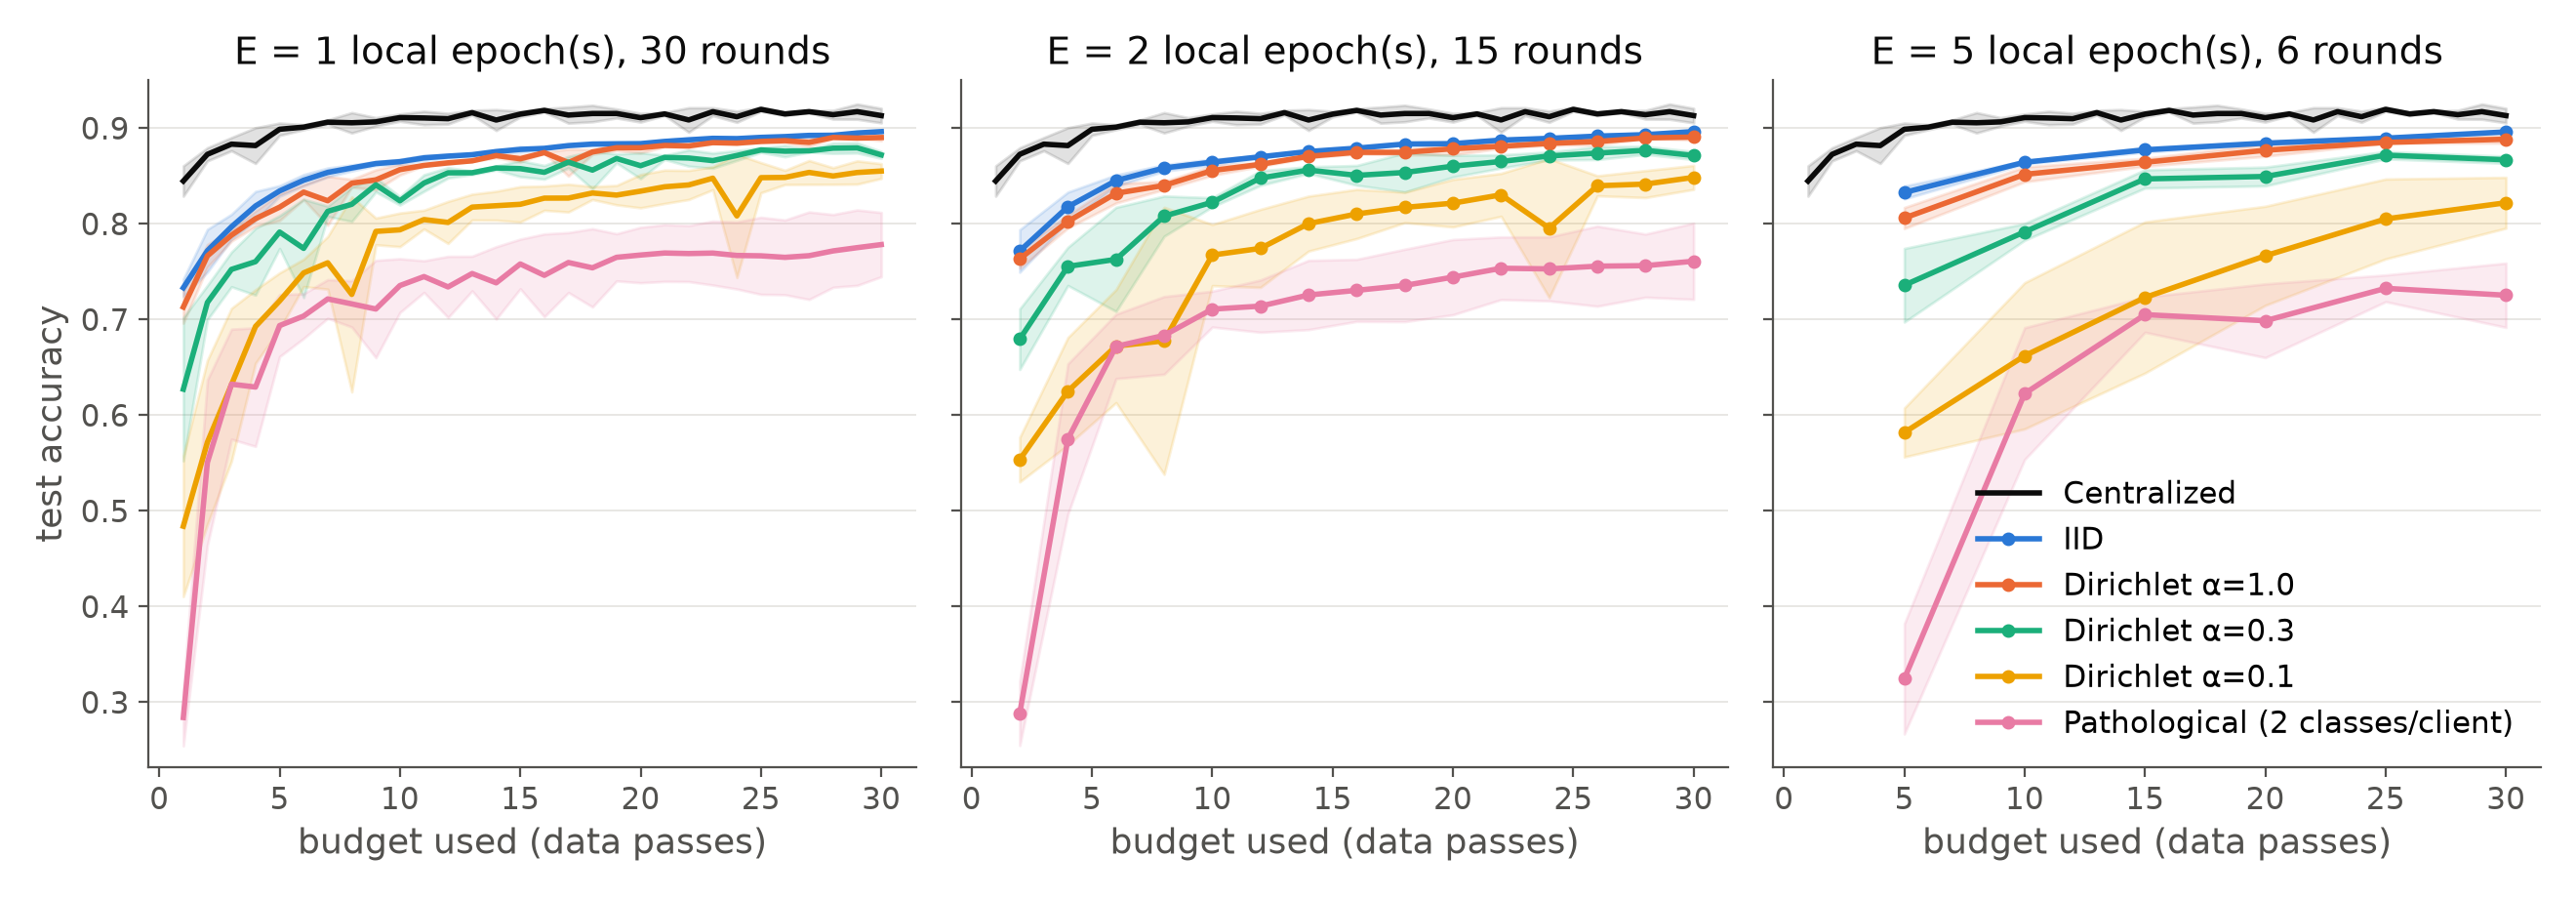
\includegraphics[width=1.00\linewidth]{figures/q2_fig1.png}
\caption*{\small \textbf{Fig. 2.} Test accuracy vs training budget for E = 1, 2, 5 local epochs (mean $\pm$ sd, 3 seeds). Black = centralized baseline.}
\end{figure}
\begin{figure}[H]\centering
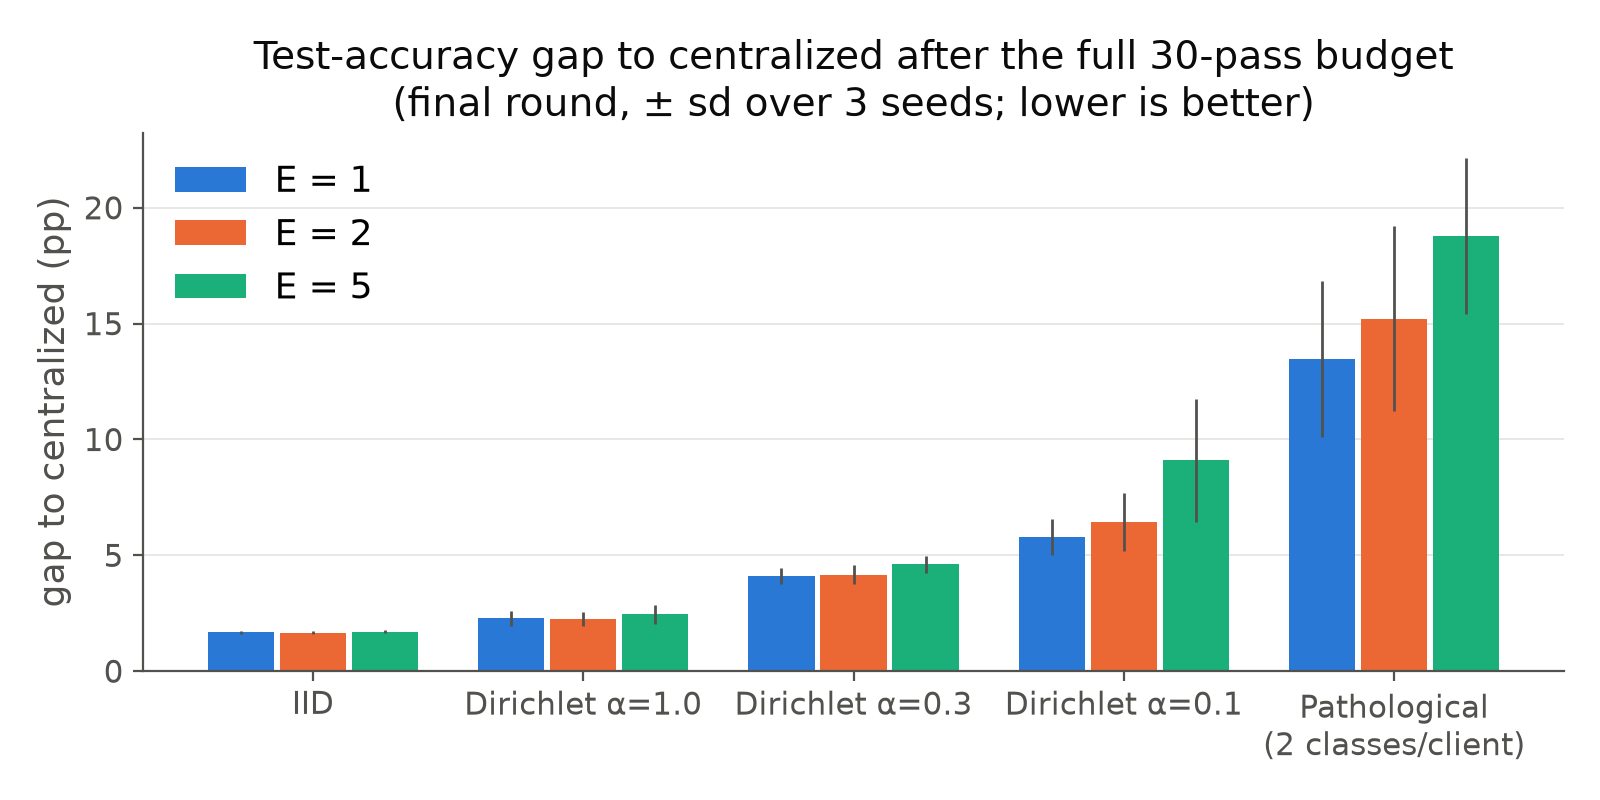
\includegraphics[width=0.80\linewidth]{figures/q2_fig2.png}
\caption*{\small \textbf{Fig. 3.} Accuracy gap to centralized after the full 30-pass budget, by data split and local epochs.}
\end{figure}
\subsection*{Findings}
\begin{itemize}
\item \textbf{When FL approaches centralized:} with IID or mildly skewed data FedAvg is within 1.7--2.5 pp of centralized (91.3\%).
\item \textbf{Communication:} E = 5 needs 5$\times$ less communication (202 vs 1,012 MB) at no accuracy cost under IID data.
\item \textbf{Heterogeneity hurts convergence:} the gap grows to 4--5 pp ($\alpha$ = 0.3), 6--9 pp ($\alpha$ = 0.1) and 13--19 pp (2 classes/\allowbreak{}client); curves oscillate and 85\% is reached late or never.
\item \textbf{Client drift:} more local epochs help under IID but hurt under skew ($\alpha$ = 0.1: 85.5\% at E=1 $\rightarrow$ 82.2\% at E=5).
\item \textbf{Privacy:} raw images never leave the clients, but this is \textbf{not} privacy. From one client update the server inferred which classes the client holds via the output-layer bias change (class-presence AUC: Dirichlet $\alpha$=1.0 0.94, Dirichlet $\alpha$=0.3 0.98, Dirichlet $\alpha$=0.1 1.00, Pathological 1.00).
\item FedAvg gives no formal guarantee; it needs secure aggregation and differential privacy (Q3).
\end{itemize}
\section*{3. Differentially Private CNN Training (DP-SGD)}
\subsection*{Method}
\begin{itemize}
\item \textbf{Training:} same CNN; 20 epochs, SGD (lr 0.05, momentum 0.9), expected batch B = 256 with Poisson sampling.
\item \textbf{Implemented from scratch:} per-example gradients (torch.func vmap) $\rightarrow$ clipping $\bar{g}$\textsubscript{i} = g\textsubscript{i}$\cdot$min(1, C/\allowbreak{}$\|$g\textsubscript{i}$\|$\textsubscript{2}) $\rightarrow$ noisy average $\tilde{g}$ = (1/\allowbreak{}B)($\Sigma$$\bar{g}$\textsubscript{i} + N(0, $\sigma$\textsuperscript{2}C\textsuperscript{2}I)).
\item \textbf{Verified:} clipped sum matches a manual loop (error \textless{}10\textsuperscript{$-$8}); noise sd = $\sigma$C.
\item \textbf{Privacy accounting:} own R\'enyi-DP accountant for the subsampled Gaussian ($\delta$ = 10\textsuperscript{$-$5}), identical to Opacus to 10\textsuperscript{$-$12}.
\item \textbf{Grid:} $\sigma$ $\in$ \{0.5, 1, 2, 4\} $\times$ C $\in$ \{0.5, 2, 8\} + clip-only + non-private baseline, 3 seeds.
\item \textbf{Membership inference:} loss-threshold attack (training members vs held-out test images).
\end{itemize}
{\scriptsize\setlength{\tabcolsep}{3pt}
\begin{longtable}{>{\raggedright\arraybackslash}p{0.209\linewidth}>{\raggedright\arraybackslash}p{0.096\linewidth}>{\raggedright\arraybackslash}p{0.096\linewidth}>{\raggedright\arraybackslash}p{0.032\linewidth}>{\raggedright\arraybackslash}p{0.032\linewidth}>{\raggedright\arraybackslash}p{0.137\linewidth}>{\raggedright\arraybackslash}p{0.161\linewidth}>{\raggedright\arraybackslash}p{0.121\linewidth}}
\toprule
\textbf{Setting (N=60k, 20 epochs)} & \textbf{$\varepsilon$ ($\delta$=10\textsuperscript{-5})} & \textbf{Acc. \% C=0.5} & \textbf{C=2} & \textbf{C=8} & \textbf{Test loss (C=0.5)} & \textbf{Train time s (C=0.5)} & \textbf{MIA AUC (C=0.5)} \\
\midrule\endhead
non-private & $\infty$ & 91.5 &  &  & 0.41 & 13 & 0.523 \\
clip only ($\sigma$=0) & $\infty$ & 84.7 & 88.5 & 91.7 & 0.85 & 42 & 0.505 \\
$\sigma$ = 0.5 & 14.28 & 84.6 & 86.2 & 81.3 & 0.86 & 30 & 0.505 \\
$\sigma$ = 1 & 1.76 & 84.1 & 81.5 & 54.5 & 0.93 & 37 & 0.506 \\
$\sigma$ = 2 & 0.62 & 81.6 & 71.1 & 10.2 & 1.55 & 42 & 0.505 \\
$\sigma$ = 4 & 0.27 & 73.4 & 50.9 & 27.1 & 5.52 & 52 & 0.506 \\
\bottomrule
\end{longtable}}
\begin{figure}[H]\centering
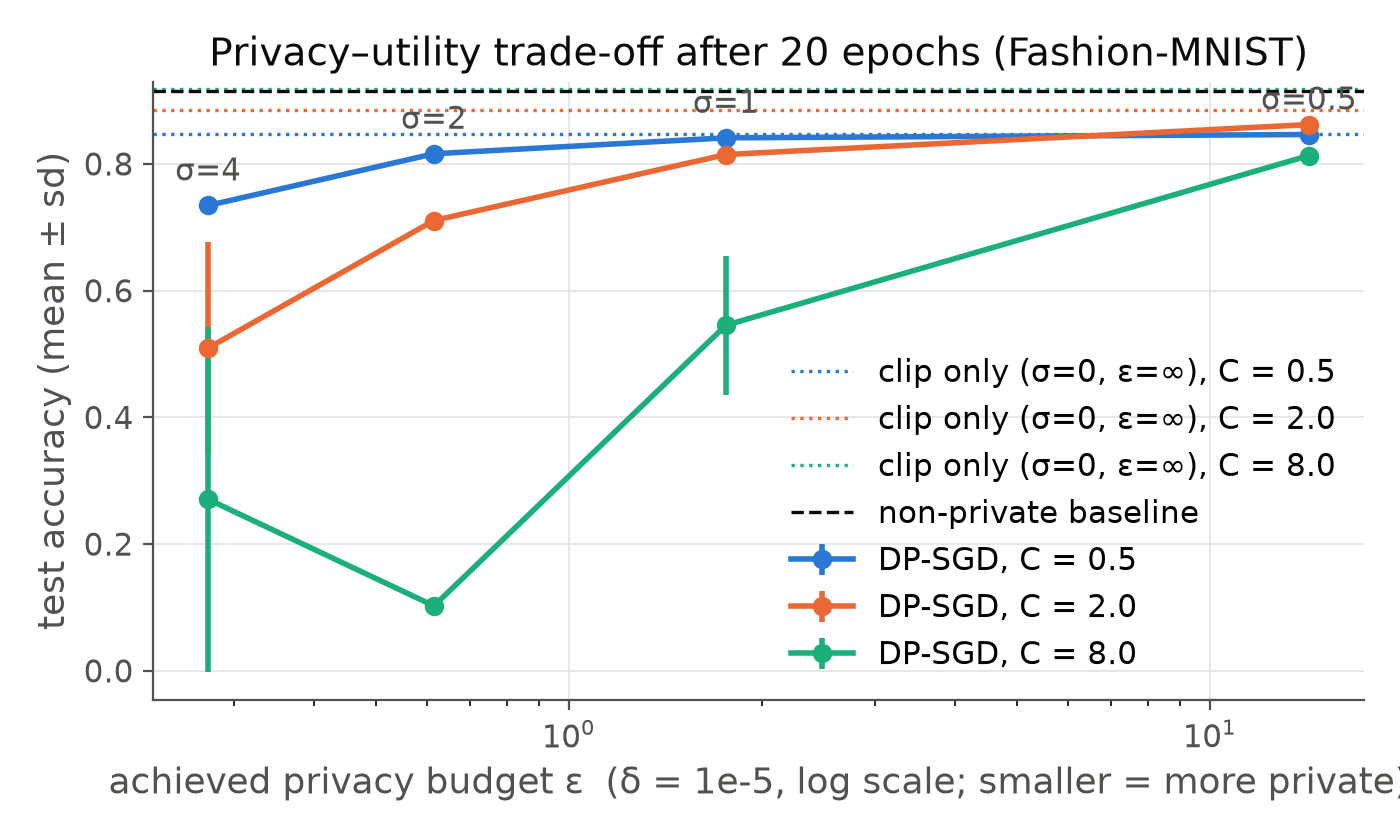
\includegraphics[width=0.82\linewidth]{figures/q3_fig1.png}
\caption*{\small \textbf{Fig. 4.} Test accuracy vs achieved privacy budget $\varepsilon$ (log scale) for each clipping norm; dotted = clip only, dashed = non-private.}
\end{figure}
\subsection*{Findings}
\begin{itemize}
\item \textbf{More noise} $\rightarrow$ stronger guarantee ($\varepsilon$ 14.3 $\rightarrow$ 1.76 $\rightarrow$ 0.62 $\rightarrow$ 0.27) and lower accuracy (84.6 $\rightarrow$ 73.4\% at C = 0.5; non-private 91.5\%). $\varepsilon$ $\approx$ 1.8 costs about 7 pp; convergence is slower and plateaus lower.
\item \textbf{Small C} biases the update (clip-only C = 0.5: 84.7\%).
\item \textbf{Large C} keeps the gradient but the noise $\sigma$C overwhelms it (C = 8 with $\sigma$ $\geq$ 1 fails to train).
\item \textbf{Best C shrinks as $\sigma$ grows} (C = 2 best at $\sigma$ = 0.5, C = 0.5 for $\sigma$ $\geq$ 1).
\item \textbf{Test loss} rises with noise (0.41 non-private $\rightarrow$ 0.93 at $\sigma$ = 1 $\rightarrow$ 5.52 at $\sigma$ = 4, C = 0.5): noisy models become poorly calibrated.
\item \textbf{Training time:} 12.5 s for the non-private model vs 21--57 s for DP (1.7--4.6$\times$ slower), because every example's gradient is computed and clipped separately. Optimiser for all runs: SGD, lr 0.05, momentum 0.9, batch 256, 20 epochs.
\end{itemize}
\begin{figure}[H]\centering
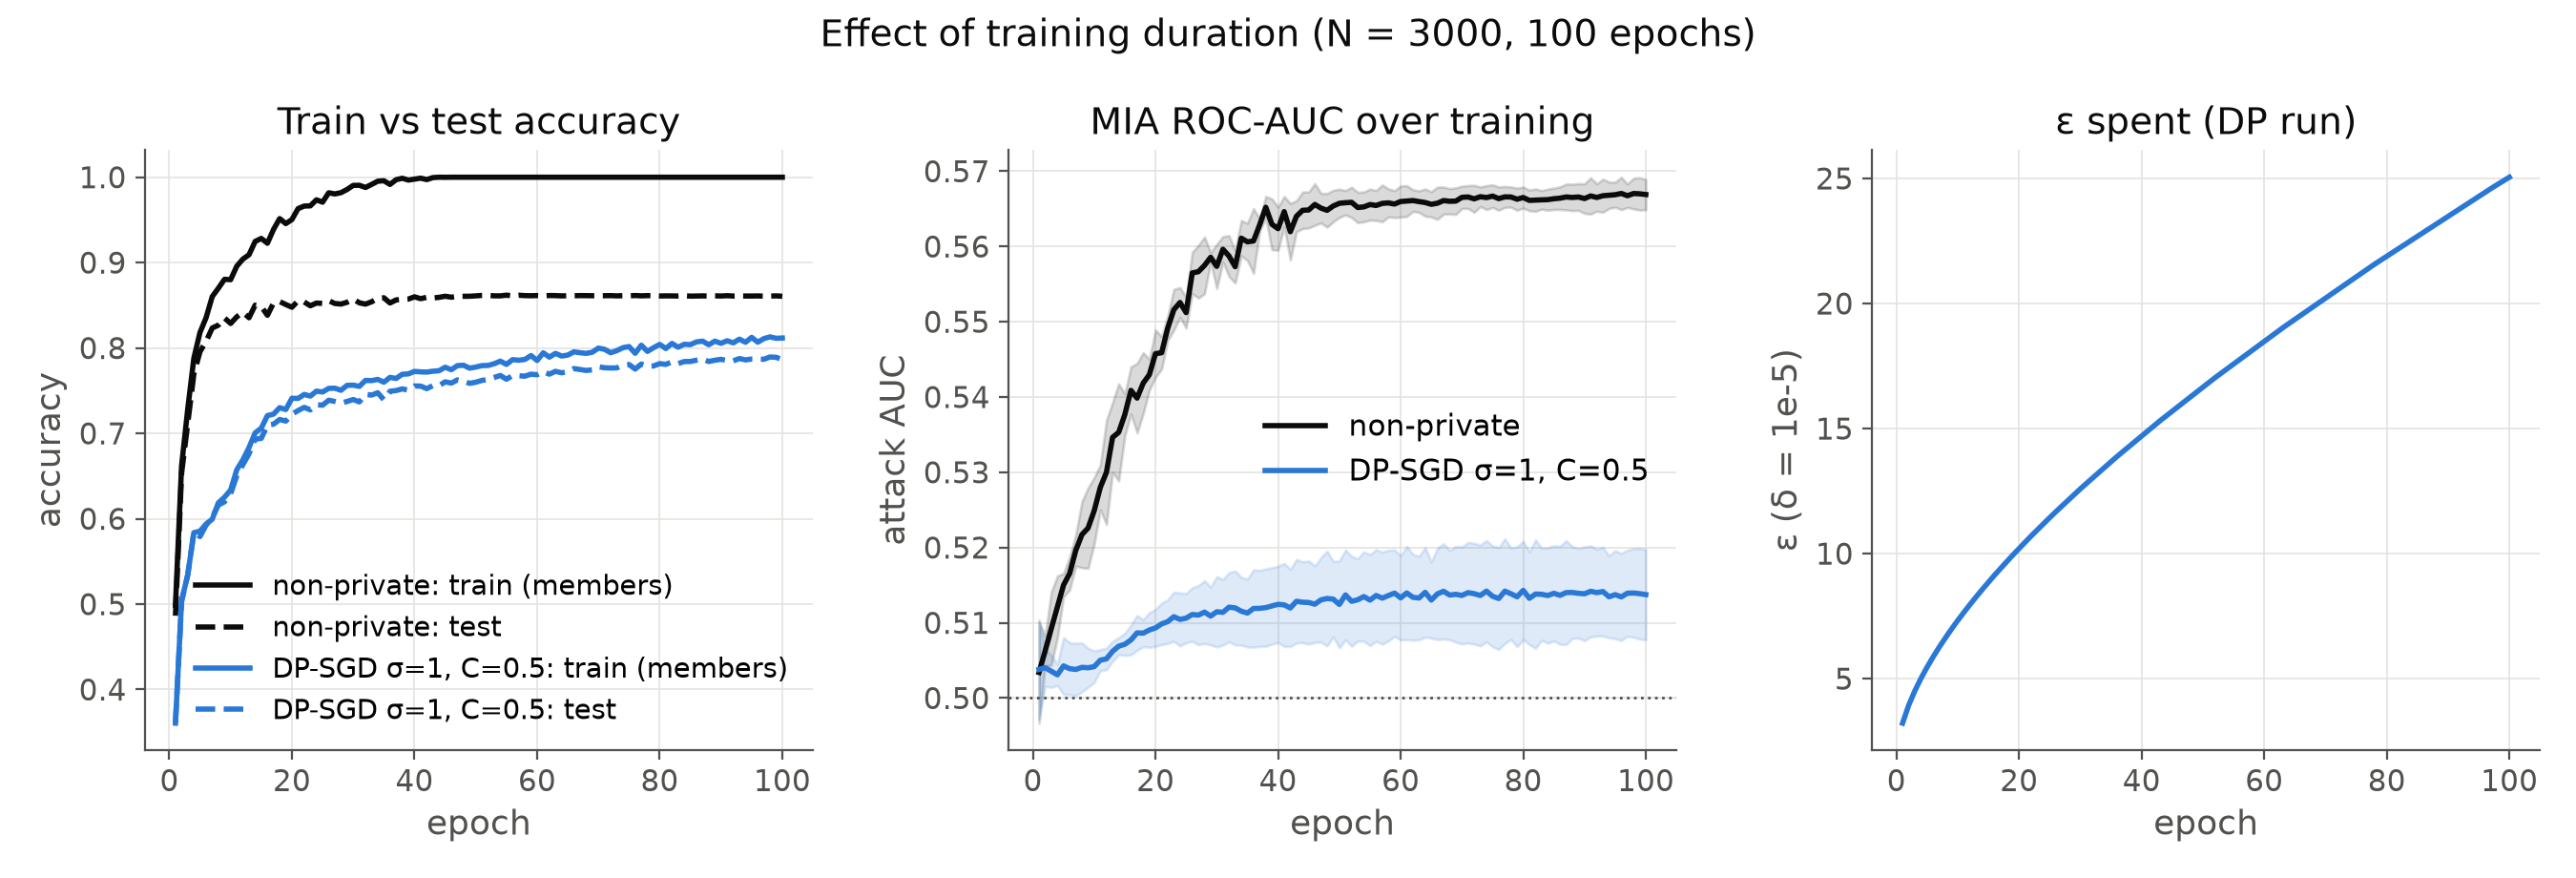
\includegraphics[width=1.00\linewidth]{figures/q3_fig6.png}
\caption*{\small \textbf{Fig. 5.} Training duration (N = 3,000, 100 epochs): train vs test accuracy, membership-inference AUC, and $\varepsilon$ spent by the DP run ($\sigma$ = 1, C = 0.5).}
\end{figure}
{\small \textbf{Dataset size and duration} (non-private /\allowbreak{} DP with $\sigma$ = 1, C = 0.5; 20 epochs unless stated):}

{\footnotesize\setlength{\tabcolsep}{3pt}
\begin{longtable}{>{\raggedright\arraybackslash}p{0.176\linewidth}>{\raggedright\arraybackslash}p{0.259\linewidth}>{\raggedright\arraybackslash}p{0.102\linewidth}>{\raggedright\arraybackslash}p{0.130\linewidth}>{\raggedright\arraybackslash}p{0.120\linewidth}>{\raggedright\arraybackslash}p{0.120\linewidth}}
\toprule
\textbf{Training-set size N} & \textbf{Test acc. \% (non-priv. /\allowbreak{} DP)} & \textbf{$\varepsilon$ of DP run} & \textbf{Train$-$test gap} & \textbf{MIA AUC} & \textbf{MIA advantage} \\
\midrule\endhead
3,000 & 84.8 /\allowbreak{} 72.2 & 10.20 & 0.103 /\allowbreak{} 0.019 & 0.546 /\allowbreak{} 0.509 & 0.109 /\allowbreak{} 0.001 \\
10,000 & 88.0 /\allowbreak{} 77.4 & 5.00 & 0.093 /\allowbreak{} 0.010 & 0.534 /\allowbreak{} 0.508 & 0.098 /\allowbreak{} 0.005 \\
30,000 & 90.5 /\allowbreak{} 81.9 & 2.61 & 0.083 /\allowbreak{} 0.008 & 0.525 /\allowbreak{} 0.506 & 0.093 /\allowbreak{} 0.013 \\
60,000 & 91.5 /\allowbreak{} 84.1 & 1.76 & 0.072 /\allowbreak{} 0.009 & 0.523 /\allowbreak{} 0.506 & 0.083 /\allowbreak{} 0.011 \\
3,000 (100 epochs) & 86.1 /\allowbreak{} 78.6 & 25.05 & 0.139 /\allowbreak{} 0.025 & 0.567 /\allowbreak{} 0.514 & 0.246 /\allowbreak{} 0.022 \\
\bottomrule
\end{longtable}}
\begin{itemize}
\item \textbf{Membership inference:} at N = 60k even the non-private model leaks little (AUC 0.523); with DP the attack is at chance (0.50--0.51), always below the DP bound.
\item \textbf{Training duration:} 100 epochs on 3,000 images lets the non-private model memorise (train 100\%, test 86\%; attack AUC 0.567, advantage 0.246). DP keeps the attack near chance (0.514), but $\varepsilon$ keeps growing with every step (25 after 100 epochs).
\item \textbf{Dataset size:} smaller N means a larger sampling rate, so $\varepsilon$ rises (1.76 at 60k $\rightarrow$ 10.2 at 3k) and DP accuracy falls, exactly where non-private models leak most.
\item \textbf{Caveats:} learning rate not tuned per C; the loss-threshold attack is weak (stronger attacks would leak more); $\varepsilon$ covers the model weights only, not the logged training statistics or the choice of C made on private data.
\end{itemize}
\section*{AI use}
\begin{itemize}
\item \textbf{Model:} Claude Opus 5.5 (Anthropic), used to generate all code and both reports.
\item The 20 Q1 audit prompts are my own and were used verbatim; the indicators and analysis code were generated by the model.
\item An independent review of all three questions was run by sub-agents of the same model; its findings were verified against the data and fixed.
\item Outputs were checked with unit tests, an Opacus cross-check of the accountant and a manual per-example clipping test.
\end{itemize}
\end{document}
